\documentclass[12pt]{article}
\usepackage{authblk}
\usepackage{amsmath}
%line2
\usepackage{amssymb}
\usepackage{amsfonts}
\usepackage{graphicx}
\usepackage{caption}
%\usepackage{subcaption}
\usepackage{subfigure}
\usepackage{setspace}
\doublespacing
\usepackage{verbatim}
\usepackage{psfrag}
\usepackage{tikz}
\usepackage{float}

\usepackage[natbibapa]{apacite}

\DeclareMathOperator*{\argmin}{\arg\!\min}
\DeclareMathOperator*{\argmax}{\arg\!\max}

\newtheorem{theorem}{Theorem}
\newtheorem{acknowledgement}[theorem]{Acknowledgement}
\newtheorem{algorithm}[theorem]{Algorithm}
\newtheorem{axiom}[theorem]{Axiom}
\newtheorem{case}[theorem]{Case}
\newtheorem{claim}[theorem]{Claim}
\newtheorem{conclusion}[theorem]{Conclusion}
\newtheorem{condition}[theorem]{Condition}
\newtheorem{conjecture}[theorem]{Conjecture}
\newtheorem{corollary}{Corollary}
\newtheorem{criterion}[theorem]{Criterion}
\newtheorem{definition}[theorem]{Definition}
\newtheorem{example}[theorem]{Example}
\newtheorem{exercise}[theorem]{Exercise}
\newtheorem{Lemma}{Lemma}
\newtheorem{notation}[theorem]{Notation}
\newtheorem{problem}[theorem]{Problem}
\newtheorem{Proposition}{Proposition}

\usepackage[margin=1in]{geometry}
\renewcommand{\abstractname}{ABSTRACT}

\begin{document}
\title{Optimal Fee Structures of Crowdsourcing Platforms}
%\author{Zhong Wen \thanks{Email: \texttt{wenzh@sem.tsinghua.edu.cn}; Corresponding author}}
%\author{Lihui Lin}
%\affil{School of Economics and Management, \\
%Tsinghua University, Beijing, 100084}
%\thanks{The work was partly supported by the National Natural Science Foundation of China (71172012,71272029).}
\author{}
\date{ }
\maketitle

%\affil{School of Economics and Management, \\
% Tsinghua University, Beijing, 100084} %\thanks{The work was partly supported by the National Natural Science Foundation of China (71172012,71272029).}

\begin{abstract}
Crowdsourcing platforms specialize in hosting open contests and usually charge a percentage of the prize as service fees. While prior research has studied the design of contests and the behavior of contestants, the strategy of a crowdsourcing platform has remained largely unexplored. We develop a game-theoretic model of crowdsourcing services and find the optimal fee structure of a platform. We prove for the case of a single contest that the service fees should be an increasing concave function of task prizes and show that this also holds true for the case of multiple contests. We further find that for a platform with many users and tasks, there is an optimal ratio of the number of contestants and contests. Our research is one of the first to focus on the strategies of crowdsourcing platforms and our results have interesting managerial implications. We show that the linear fee schedule widely used in practice is not optimal and that a platform is better off lowering the fee rate for contests with high prizes. It is also in the best interests of a platform to develop both sides of the crowdsourcing market proportionally and keep the ratio of contestants and contests at the optimal level.

Keywords: Crowdsourcing; E-Commerce; Mechanism design
\end{abstract}

\section{Introduction}

Crowdsourcing refers to the act of outsourcing tasks to an undefined
Internet community in an open call (\citet{Howe:2006}). Enabled by
Web 2.0 technologies, crowdsourcing allows companies to leverage the
global Internet community to complete tasks traditionally performed
by employees or contractors. Traditionally, Internet users are mainly
viewed as consumers and companies focus on marketing efforts to reach
them; with the development of participatory social media technologies
users are increasingly engaged in the production side of the economy,
providing solutions to problems, creating content, and collaborating
on projects. To harness the productivity and creativity of the Internet
community at large new business models have proliferated in recent
years and crowdsourcing is one of the most promising approaches among
them (\citet{Brabham:2013}).

To tap into the online crowds, many companies have launched their
own crowdsourcing initiatives, often to improve products and services.
For example, Netflix held an open competition for the best collaborative
filtering algorithm to predict user ratings for films and the grand
prize of \$1,000,000 was awarded to the winning team in September
2009. Dell and Starbucks have established their online communities
(IdeaStorm.com and MyStarbucksIdea.com, respectively) focusing on
ideation for open innovation, where customers are called upon to share,
discuss, evaluate, and develop ideas that may lead to better products
and services.

In addition to companies' crowdsourcing projects, more noteworthy
is the advent of crowdsourcing organizations: entities with crowdsourcing
as their core business \citep{Hempel:2006, Howe:2006, Saxton:2013}.
Based on a comprehensive empirical study of more than 100 crowdsourcing
organizations, \citet{Saxton:2013} identify nine major business models
of crowdsourcing, including the intermediary model (e.g., InnoCentive,
Topcoder, Amazon's Mechanical Turk), product design model (e.g., Threadless.com),
and knowledge base building (e.g., Wikipedia.org). In this paper,
we focus on platforms that adopt the intermediary
business model, where web users find tasks posted by solution seekers
on the platform, complete and submit their work, and potentially earn
from the seekers, while the platform provides services including facilitating
transactions and communication and addressing intellectual property
issues. By attracting task-posters and solvers to the same platform,
crowdsourcing websites create a kind of freelance markets that were
once forecast by \citet{Malone:2004}.

These platforms are usually independent, for-profit businesses, making
money by charging service fees for organizing crowdsourcing tasks.
InnoCentive is one of the most prominent crowdsourcing intermediaries
focusing on open innovation, where companies seek solutions to problems
in domains such as engineering, computer science, math, life sciences,
physical sciences, and businesses. As of August 2013, InnoCentive
has a total of more than 300,000 registered solvers. It has organized
more than 1,650 external challenges with a success rate of 85\%. The
awards ranged from \$5,000 to more than \$1 million based on the complexity
of the problem and nature of the contest, and more than \$40 million
in total has been posted as award money. Crowdspring.com, for another
example, is one of the largest marketplaces for graphic design (e.g.,
logo), web design, and other creative tasks. As of February 2014,
projects have received more than 4.8 million entries in total, with
120 entries per project on average. Crowdsourcing is also fast growing
globally. For example, Zhubajie is one of the biggest crowdsourcing
platforms in China, posting a large variety of tasks such as problem
solving, design, website development, and writing and multimedia services.
With more than 9 million registered professionals, its total transaction
amount reached \$520 million in February 2014.

The emergence of crowdsourcing platforms presents new challenges to
the design of crowdsourcing tasks. When a firm (called the contest
sponsor) organizes a crowdsourcing contest without an intermediary,
it gleans all the benefit of the results and the firm will set an
optimal prize accordingly (e.g., Netflix's open challenge). When using
an intermediary, however, the contest sponsor's optimal prize is now
distorted by the service fee schedule charged by the intermediary
(e.g., InnoCentive). These platforms usually charge a service fee
as a percentage of the reward of the tasks. For example, InnoCentive
charges contest sponsors a \$15,000 posting fee upfront and receives
a commission on prizes for those challenges where awards were given.
Service fees account for 40\% of a seeker company's total payment
to Crowdspring.com while Zhubajie.com charges a uniform 20\% of prizes
as service fees. However there is little research on the optimal fee
schedule of a crowdsourcing platform.

This research focuses on the pricing strategy of a crowdsourcing intermediary.
A crowdsourcing platform (hence called platform) faces the following
tradeoff: a higher commission rate means it receives higher revenues
from a challenge (if successfully completed); however, it may discourage
the sponsors from setting high prizes in the first place and furthermore
a steep fee schedule may price certain sponsors out of the market.
Therefore, for the platform, a central question is: what is the
optimal fee schedule that maximizes its own profit, given the task
sponsors' incentives? This constitutes the key research question of
this study.

We develop a game-theoretic model of crowdsourcing services
and find the properties of the optimal fee schedule charged by a platform.
We model the platform's problem as a classic mechanism design
problem. The platform as the principal seeks to design a fee schedule
that maximizes its expected profit. Contest sponsors then choose a proper prize
for their contests that motivates contestants to provide solutions.
In our setting, contest sponsors post crowdsourcing challenges where
the top solution will be selected, awarded, and often adopted immediately
with little modification. This type of challenges is often referred
to as research tournaments in the literature (\citet{Moldovanu:2001}) and suitable for sponsors who are interested
in maximizing the quality of the top solution. Most design tasks and
challenges involving scientific research belong to this category%
\footnote{In contrast, in another type of challenges called consumer contests,
the contest sponsor's goal is to maximize the total quality of all
solutions. One example of a consumer contest is ideation, which is
a global brainstorm for producing a breakthrough idea and the contest
sponsor of an ideation task is interested in generating many good
ideas (e.g., \cite{Leim:2009}).%
}.

We first consider the case where the platform hosts a single contest in which contestants can participate. We study the equilibrium strategies for the contestants and the contest sponsor, as well as the optimal fee schedule for the platform. We then extend our model to examine the case where the platform hosts multiple contests. One of the major strengths of crowdsourcing intermediaries is that they specialize in organizing challenges and they build a two-sided market by bringing both seekers and solvers together. More solvers are attracted to a platform as it hosts more contests and vice versa. This gives rise to more research questions: Is the optimal fee schedule we propose sensitive to the case of multiple contests? Furthermore, as a platform grows and gains popularity, which side of the market should it focus on? Should it recruit more solvers or host more challenges?

Our attempt to answer these questions yields some interesting results. First, we find that the presence of a crowdsourcing platform distorts sponsors' strategies, causing them to set lower prizes. Second, our results suggest that a linear fee schedule, which is widely adopted in the industry, is not optimal. Instead, the optimal service fees charged by the crowdsourcing platform should be an increasing concave function of contest prizes in a single contest setting. This means the platform's optimal fee schedule encourages sponsors with strong preference for solution quality (called the high type sponsors) to set high prizes; in other words, the optimal schedule distorts high type sponsors' prizes less. Furthermore, sponsors with low preference for quality might be priced out of the market. Third, we find that when a platform hosts multiple contests simultaneously, in which a large number of solvers can choose to participate, a sponsor can set the prize by focusing on his own preference for quality without concerning the prizes set by others. Fourth, we demonstrate that for a platform with multiple contests and many solvers, its optimal fee schedule has similar properties as that in a single contest setting. Lastly, we find that for a given number (sufficiently large) of solvers there exists an optimal number of contests a platform should host.

Our research focuses on the mechanism design of crowdsourcing platforms, which, as far as we know, has not been explored in the literature. Prior research on crowdsourcing has mostly studied either the strategies
of the contest sponsors or the behavior of contestants (see, among
others, \citep{Archak:2009, Chawla:2011, Ghosh:2012, Huang:2013, Liu:2013}),
and to our best knowledge, no previous studies in crowdsourcing have
considered the optimal fee schedules of crowdsourcing platforms.

Extant theoretical research on crowdsourcing mostly concerns the contest
sponsor's optimal strategies. One of the key issues studied is the
optimal division of prize budgets and the asymptotic structure of
the crowdsourcing contests \citep{Archak:2009, Chawla:2011, Ghosh:2012}.
\citet{DiPalantino:2009} presents an interesting model that considers
the competition between contests. The empirical literature
on crowdsourcing largely concentrates on the behavior of task solvers. \citet{Yang:2008}
examine the user behavior patterns on Taskcn.com and find that a small
core group of users propose nearly 20\% of the winning solutions on
the site. Related studies on knowledge sharing websites also focus
on user behavior patterns and find that user participation and contribution
are highly skewed on various knowledge sharing websites \citep{Adler:2007, Golder:2006, Welser:2007}. \citet{Huang:2013}
presents empirical evidence on how incentive structures offered by
the contest sponsor could affect the quality of the solutions produced
in crowdsourcing contests. They develop a dynamic structural model
of user participation in crowdsourcing contests and using data from
Threadless.com they find that participants put in less effort as competition
for the award increases. \citet{Liu:2013} study the effects of incentives
on solvers in crowdsourcing contests and through field experiments
they find that higher rewards induce more participation and higher
quality submission, but early entry of a high-quality submission may
result in lower quality in sequential contests. While our research
builds on the existing literature, our focus on the strategy of crowdsourcing
platforms is unique.

Our paper draws from the economics literature on contest design and
mechanism design. There is a voluminous economics literature on contest
design. \citet{Wright:1983}, \citet{Taylor:1995} and \citet{Fullerton:1999}
study various models of research tournaments where a unique prize
is awarded. \citet{Lazear:1981} and \citet{Nalebuff:1983} emphasize
the use of relative compensation tournaments in order to extract effort.
\citet{Krishna:1998} study the optimal allocation of prizes in contests
with two, three, or four contestants. \citet{Moldovanu:2001} and
\citet{Moldovanu:2006} study the optimal allocation of prizes. The
contest design part of our model is based on their work. The methodology
we use for solving the fee-schedule game is from the classic mechanism
design literature \citep{Baron:1982, Guesnerie:1984}. The point of
departure of this paper from the literature is that, instead of considering
the optimality of contest designs as these studies, we consider the
design of crowdsourcing platforms.


\section{Model Setup}

There are three types of players: a crowdsourcing platform, contest sponsors, and contestants.
All agents are assumed to be risk neutral and utility maximizers.
The platform attracts both contest sponsors and contestants. Contest sponsors are firms
that post tasks on the crowdsourcing platform and solicit proper solutions
in the format of a contest. Contestants (also called solvers) are individuals (or teams,
organizations, etc.) who make efforts to provide solutions and may
win a prize from the contest sponsor.

In a principal-agent setting, the platform is the principal who
designs the rules of crowdsourcing contests. The rules specify how
a crowdsourcing contest is conducted, how the winners of contests
are rewarded, and what are the service fees charged for hosting crowdsourcing
contests. We focus on the design of the service fee menu, $K(V)$,
which determines how much the platform charges a crowdsourcing
contest with winning prize $V$. Assume the cost of hosting a contest
is zero. The goal of the platform is to choose $K(V)$ to maximize
its expected profits from organizing contests.

Contest sponsors choose prizes to maximize their expected utility
from task solutions. Contest sponsors are characterized by their private
information $\theta$, which measures how much the sponsors value
the quality of the solutions. $\theta$ is a random variable drawn
from a cumulative distribution function $G$ with support $[\underline{\theta},\overline{\theta}]$,
which is common knowledge. Given the service fee menu $K(V)$, a contest
sponsor chooses prize $V$ for its contest. $V$ will be rewarded
to the winning contestant.

Contestants choose private efforts spent on contests, given other
contestants' efforts and contest prizes. The set of contestants is
${\cal N}$$=\{1,2,\cdots,n\}$. Contestants are privately endowed
with $s_{i}$, which is a skill level measure that transforms effort
to disutility. Low $s_{i}$ means contestant $i$ has a high skill
level (i.e., lower disutility for the same effort) and vice versa.
$s_{i}$ are drawn independently from a common cumulative distribution
function $F$ with support $[\underline{s},\overline{s}]$, where
$\overline{s}>\underline{s}>0$. The density function, $f$, is continuous
and positive. We assume $\underline{s}>0$ to avoid the possibility
that the highest skill type makes an infinite effort. We assume the
contestants do not know the efforts made by others, which meanrs that efforts can
be thought undertaken simultaneously. The disutility from effort $e$
for a contestant endowed with $s$ is $sc(e)$, where $c$ is a strictly
increasing convex function with $c(0)=0,c'(e)>0,c''(e)>0$. A contestant
cannot recoup his effort if he does not win any prize. Therefore a contestant's payoff is either $V-sc(e)$ if he wins the prize $V$,
or $-sc(e)$ if he loses.

The type of contest we study is called research tournaments, where the sponsor values only the solution with the highest quality, which will be selected and awarded. Thus, the sponsor's utility is modeled as $U(V)=\theta(\max_{i \in \cal N}Q(e_i))-V-K(V)$. $Q$ is a function that maps the contestant's effort $e$ to solution quality.
$Q$ is assumed to be deterministic and quasi-concave with each contestant's
effort level, that is, a higher effort leads to higher quality, but
the marginal effort has a non-increasing return.

The timing of events is as follows: first the platform announces
its fee schedule $K(V)$, then contest sponsors choose the prize $V$,
after which the contestants make efforts and submit their solutions.
We first consider the case of a single contest, and then examine the
case of multiple contests where contestants can choose to participate
in any of the contests and the platform maximizes its total revenues
from all contests.


\section{Single Contest}

In this section, we consider a basic model where the platform hosts only one contest. In this setting, the contestants' game is essentially an all-paid auction with incomplete information. We solve the game by backward induction: we first analyze the contestants' strategy, and then study the strategies of the sponsor and the platform.


\subsection{Contestants' Strategy}

By the revelation principle, we only need to consider the truth-revealing
strategy. We denote the equilibrium effort strategy by $e(s)$, which
maps contestant type $s$ to his effort $e(s)$. Assume that all contestants
undertake efforts according to $e(\cdot)$, and assume that this function
is strictly monotonic and differentiable. The maximization problem
of a contestant of type $s$ reads:
\begin{equation}
\pi(s)=\max_{x}[V(1-F(e^{-1}(x)))^{n-1}-sc(x)],
\end{equation}
where $(1-F(e^{-1}(x)))^{n-1}$ is the probability of winning prize
$V$.

Previous studies \citep{Moldovanu:2001, Archak:2009} show that this
type of game has a unique pure-strategy symmetric Bayes-Nash equilibrium:

\begin{equation}
e(s)=c^{-1}(VA(s)), \text{where } A(s)=(n-1)\int_{s}^{\overline{s}}\frac{1}{t}(1-F(t))^{n-2}f(t)dt.\label{def_A}
\end{equation}
Note that $e(\overline{s})$=0, the contestant with the lowest skill
level exerts zero effort. Since $A'(s)<0$, we have $e'(s)=c^{-1'}VA'(s)<0$.
The equilibrium effort increases with the skill of contestants.

The solution quality could be written as a function of contestant
effort, that is, $Q(e(s,V))=Q(c^{-1}(VA(s)))$. Since $Q(e)$ is quasi-concave
and $c(e)$ is convex, $Q(s,V)$ must be a concave function of $V$.

The contest sponsor is interested in the solution with the highest quality. Define $q(V)$ as the highest expected quality induced by prize $V$. We have the following proposition:

\begin{Proposition}\label{qV}
The expected top quality induced by prize $V$ in a contest is
\[
q(V)=\int_{\underline{s}}^{\overline{s}}Q\left(c^{-1}\left(V\int_{s}^{\overline{s}}\frac{(n-1)(1-F(t))^{n-2}f(t)}{t}dt\right)\right)n\left(1-F(s)\right)^{n-1}f(s)ds
\]
\end{Proposition}
(See Appendix for proof.)

Proposition \ref{qV} shows that the highest expected quality comes from the contestant with the highest skills participating in the contest. Note that by the concavity of $Q$, $q(V)$ must be a concave function of $V$
as well.


\subsection{The Platform's Optimal Strategy}

Now consider the contest sponsor's problem. With the definition of $q(V)$, the sponsor's objective can be written as

\begin{equation}
\max_{V}U(V)=\max_{V}   \theta q(V)-V-K(V)
\end{equation}


Given the fee schedule $K(V)$, sponsor $\theta$ is self-assigned
to the optimal prize $V(\theta)$ that maximizes his utility. $V(\theta)$
should satisfy the first-order condition
\begin{equation}
\theta q'(V)-1-K'(V)=0.\label{prize}
\end{equation}


Not knowing the sponsor's type, the platform's objective is to
offer the sponsor a menu of service contracts $(V(\theta),K(V(\theta)))$
that maximizes the expected profit
\begin{equation}\label{UCSR}
\max_{K(V(\theta))}\int_{\underline{\theta}}^{\overline{\theta}}K(V(\theta))g(\theta)d\theta,
\end{equation}
subject to the incentive-compatibility (IC) and individual rationality
(IR) constraints:
\begin{align*}
\text{(IC)} & \text{ For each }\theta,\theta q(V(\theta))-V(\theta)-K(V(\theta))\geq\theta q(V(\phi))-V(\phi)\\
 & -K(V(\phi)),\text{for all}\phi\neq\theta\\
\text{(IR)} & \text{ For all }\theta,\theta q(V(\theta))-V(\theta)-K(V(\theta))\geq0
\end{align*}

Solving the above problem, we obtain the platform's optimal fee schedule.

\begin{Proposition}\label{V_solution}
The crowdsourcing platform's optimal service fee schedule is
\begin{align}
V(\theta) & =q'^{-1}(1/(\theta-1/H(\theta))), \text{where }  H(\theta)=g(\theta)/(1-G(\theta))\\
K(\theta) & =\theta q(V(\theta))-V(\theta)-\int_{\theta^{*}}^{\theta}q(V(t))dt,\\
\theta^{*} & \leq\theta<\overline{\theta}, \hat{\theta}-1/H(\hat{\theta})=1/q'(0),\theta^{*}=\max \{\underline{\theta},\hat{\theta}\}
\end{align}
\end{Proposition}

First, Proposition 2 implies that when a sponsor posts a contest, it offers a lower
prize than it would without a service fee imposed on it. Suppose the
optimal prize a sponsor chooses when there is no service fee is $V^{(1)}(\theta)$.
$V^{(1)}$ satisfies $q'(V^{(1)}(\theta))=1/\theta$. From Proposition 2, we know
\begin{equation}
q'(V(\theta))=1\Big/\Big(\theta-\frac{1}{H(\theta)}\Big).\label{csfocc}
\end{equation},
which indicates that when there is a service fee, a sponsor will choose
a smaller prize except at the upper bound, and a high type sponsor is
less affected than a low type. In particular, if $1/H(\overline{\theta})=0$
(for distribution with limit upper bound), $V(\overline{\theta})=V^{(1)}(\overline{\theta})$.

Proposition 2 shows that the optimal fee charging
type $\theta$ sponsor is
\begin{equation}
K(\theta)=\theta q(V(\theta))-V(\theta)-\int_{\theta^{*}}^{\theta}q(V(t))dt.\label{feef}
\end{equation}

Equation (\ref{feef}) indicates how servicing low type sponsors affects
the platform's profitability. A sponsor
of type $\theta$ could pay fee as much as $\theta q(V(\theta))-V(\theta)$.
However, due to the existence of sponsors with lower values of $\theta$,
equation (\ref{feef}) shows that the platform must leave information
rent as much as $\int_{\theta^{*}}^{\theta}q(V(t))dt$ to the sponsor.
Otherwise, the sponsor would choose a lower prize. Therefore, the
maximum fee that the platform can actually charge the type $\theta$
poster is $\theta q(V(\theta))-V(\theta)-\int_{\theta^{*}}^{\theta}q(V(t))dt$.

We also find:
\begin{Proposition} Under the optimal fee schedule, low-type sponsors
may choose not to post a contest with the platform. Specifically,  if $\hat{\theta}>\underline{\theta}$ where $\hat{\theta}$ is given by: $\hat{\theta}-1/H(\hat{\theta})=1/q'(0)$, then a type $\theta$ sponsor such that $\underline{\theta}<\theta<\hat{\theta}$ does not post a contest on the platform. \end{Proposition}

Proposition 3 suggests that under the optimal fee schedule, low-type sponsors
might be priced out of the market.

Now we characterize the property of $K(V)$. From Proposition 2, $K'(V)=\theta q'(V)-1=1/(\theta H-1)\geq0$.
Differentiating $K'(V)$ by $\theta$, we have
\begin{equation}
K''(V)V'(\theta)=\frac{d(1/(\theta H-1))}{d\theta}=-\frac{\theta H'+H}{(\theta H-1)^{2}}\leq0.
\end{equation}
So $K''(V)\leq0$, and $K'(V(\overline{\theta}))=0$ when $H(\overline{\theta})=\infty$.
Therefore, $K(V)$ is an increasing concave function of $V$.

Define the service fee rate by $K/V$. By the concavity of $K$, the
service fee rate decreases with the prize since
\begin{equation}
\frac{d(K/V)}{dV}=\Big(\frac{dK}{dV}-\frac{K}{V}\Big)\frac{1}{V}<0.
\end{equation}


We summarize the above results in the next proposition. \begin{Proposition}
The optimal crowdsourcing service fee is an increasing, concave function
of the contest prize, which implies that the service fee rate decreases
with the prize. \end{Proposition}

It is instructive to compare the optimal fee schedule to the linear
fee schedule used widely in industry. Proposition 4 suggests that a linear fee schedule, or a constant fee
rate is not optimal. Instead, it is optimal for the platform to
charge a lower percentage of the prize for high-prized contests.

Consider a linear fee schedule, $K(V)=kV,k>0$.
The utility of type $\theta$ sponsor is $\theta q(V(\theta))-V(\theta)-kV(\theta)$.
The first order condition yields
\begin{equation}
q'(V)=(1+k)/\theta.\label{q_linear}
\end{equation}

Define $\theta^{**}$, such that $(1+k)=1/(1-1/(\theta^{**}H(\theta^{**})))$.
Comparing equations (\ref{q_linear}) and (\ref{csfocc}), it is evident
that the sponsor $\theta$ will choose a higher prize under the optimal
fee schedule than under the linear fee schedule when $\theta>\theta^{**}$;
he will choose a lower prize under the optimal fee schedule than under
the linear fee schedule when $\theta<\theta^{**}$. The underlying
mechanism is that the optimal fee schedule is a concave function with
decreasing marginal rate, $K'(V)=1/(\theta H-1)$. Therefore, the
optimal schedule encourages/discourages the higher/lower types to
choose a higher prize. The
intuition is as follows. Lowering the service fee rate has two countervailing
effects on the platform's profit: it encourages the sponsor to
offer a higher prize while reducing the share of the prize the platform
gets. In the case of a high type sponsor, the former effect dominates
the latter, thus it pays off for the platform to lower the fee
rate. In other words, a slightly lower fee rate charged to a high-type
sponsor induces such a high prize that the platform gets higher
profits even at the lower rate. Note that the highest type sponsor
pays the highest overall service fee at the lowest fee rate.

Figure 1 (a) illustrates the prizes chosen by a sponsor of type $\theta$
under the optimal and linear fee schedules and panels (b) and (c) of Figure 1 depict the platform's optimal fee schedule as a function of sponsor type $\theta$ and of contest prize $V$ respectively.

\begin{figure}
\centering
\subfigure[]{
\begin{minipage}[t]{0.45\textwidth}
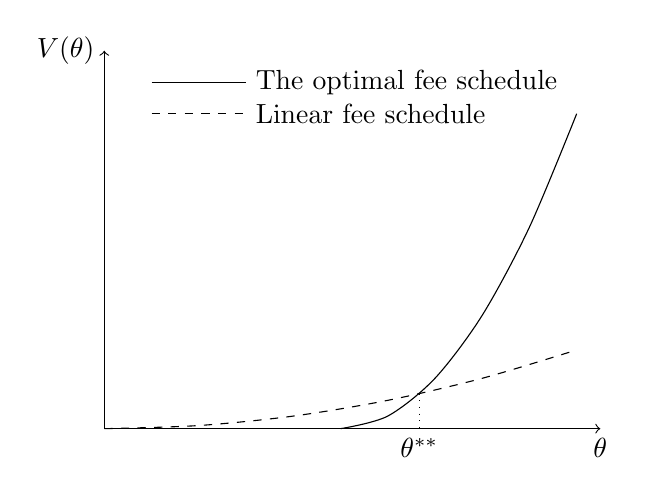
\begin{tikzpicture}[xscale=6, yscale=8]
\draw[->] (0,0) -- (1.05,0) coordinate (x axis);
\draw[->] (0,0) -- (0,0.6) coordinate (y axis);
%\draw (0,0) node [below] {$0$};
\draw (1.05,0) node [below] {$\theta$};
%\draw (1.0,0) node [below] {$1$};
\draw (0, 0.6) node [left] {$V(\theta)$};
\draw [smooth]  plot coordinates{(0.5,0)(0.6, 0.02) (0.7, 0.08) (0.8, 0.18) (0.9, 0.32) (1, 0.5)};
\draw [smooth, dashed]  plot coordinates{(0,0)(0.2, 0.005) (0.4, 0.02) (0.6, 0.045) (0.8, 0.08) (1, 0.125)};
\draw [smooth] plot coordinates {(0.1,0.55)(0.3,0.55)};
\draw  (0.3, 0.55) node [right] {The optimal fee schedule};
\draw [dashed] plot coordinates {(0.1, 0.5)(0.3,0.5)};
\draw (0.3, 0.5) node [right] {Linear fee schedule};
\draw [dotted] plot coordinates {(0.6667, 0.05556)(0.6667,0)};
\draw (0.6667,0) node [below] {$\theta^{**}$};
\end{tikzpicture}
\end{minipage}
}
\subfigure[]{
\begin{minipage}[t]{0.45\textwidth}
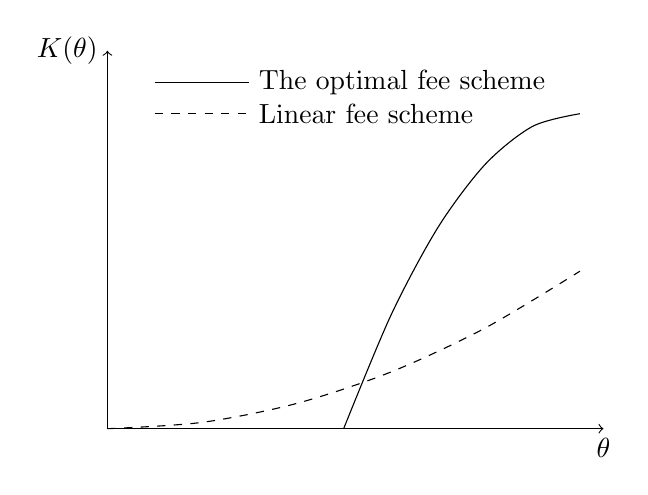
\begin{tikzpicture}[xscale=6, yscale=8]
\draw[->] (0,0) -- (1.05,0) coordinate (x axis);
\draw[->] (0,0) -- (0,0.6) coordinate (y axis);
%\draw (0,0) node [below] {$0$};
\draw (1.05,0) node [below] {$\theta$};
%\draw (1.0,0) node [below] {$1$};
\draw (0, 0.6) node [left] {$K(\theta)$};
\draw [smooth]  plot coordinates{(0.5,0)(0.6, 0.18) (0.7, 0.32) (0.8, 0.42) (0.9, 0.48) (1, 0.5)};
\draw [smooth, dashed]  plot coordinates{(0,0)(0.2, 0.01) (0.4, 0.04) (0.6, 0.09) (0.8, 0.16) (1, 0.25)};
\draw [smooth] plot coordinates {(0.1,0.55)(0.3,0.55)};
\draw  (0.3, 0.55) node [right] {The optimal fee scheme};
\draw [dashed] plot coordinates {(0.1, 0.5)(0.3,0.5)};
\draw (0.3, 0.5) node [right] {Linear fee scheme};
%\draw[domain=0:1, smooth, color=black, variable=x, samples=100] plot function{4*(-x*x+x-0.375)};
\end{tikzpicture}
\end{minipage}
}

\subfigure[]{
\begin{minipage}[t]{0.45\textwidth}
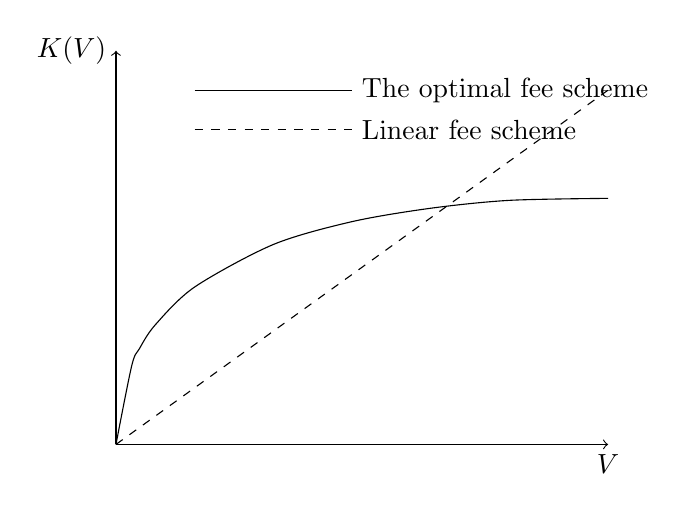
\begin{tikzpicture}[xscale=10, yscale=10]
\draw[->] (0,0) -- (0.625,0) coordinate (x axis);
\draw[->] (0,0) -- (0,0.5) coordinate (y axis);
%\draw (0,0) node [below] {$0$};
\draw (0.625,0) node [below] {$V$};
%\draw (1.0,0) node [below] {$1$};
\draw (0, 0.5) node [left] {$K(V)$};
\draw [smooth]  plot coordinates{(0,0) (0.02, 0.1) (0.03, 0.122) (0.05, 0.152 ) (0.1, 0.2) (0.2, 0.254) (0.3, 0.283) (0.4, 0.3) (0.5, 0.31) (0.625, 0.3125)};
\draw [dashed]  plot coordinates{(0,0) (0.625,0.45)};
\draw [smooth] plot coordinates {(0.1,0.45)(0.3,0.45)};
\draw  (0.3, 0.45) node [right] {The optimal fee scheme};
\draw [dashed] plot coordinates {(0.1, 0.4)(0.3,0.4)};
\draw (0.3, 0.4) node [right] {Linear fee scheme};
\end{tikzpicture}
\end{minipage}
}
\caption{Optimal Prize and Fee Functions}
\end{figure}

\subsection{An Example}

In this section, we provide an example to illustrate the nature of
the optimal fee schedule. Assume the contestant's skill measure $s$
follows a uniform distribution $U(m-b,m+b)$, and $F(s)=(s-(m-b))/(2b),f(s)=1/(2b)$.
Assume $c(e)=e^{2}$, $Q(x)=x$ and $G$ follows a uniform distribution
$U(0,1)$. Based on previous results, the highest expected quality induced by a prize of $V$ is then given by

\begin{equation}
q(V)=\sqrt{V}\int_{m-b}^{m+b}n\Big(1-\frac{t-(m-b)}{2b}\Big)^{n-1}\frac{1}{2b}\sqrt{A(s)}dt.\label{num_qV}
\end{equation}

where \[
A(s)=(n-1)\int_{s}^{m+b}\frac{1}{t}\Big(1-\frac{t-(m-b)}{2b}\Big)^{n-2}\frac{1}{2b}dt.
\]

For simplicity, we write $q(V)=\alpha\sqrt{V}$, where $\alpha$ represents
the integral in equation \ref{num_qV}. Clearly, the highest expected quality of solution depends on $\alpha$.

We then derive the optimal fee schedule for the platform. By Proposition (\ref{V_solution}),
\begin{equation}
V(\theta)=\Big(\frac{\alpha(2\theta-1)}{2}\Big)^{2},\label{num_V}
\end{equation}
\begin{equation}
K(\theta)=\alpha^{2}\Big(-\frac{\theta^{2}}{2}+\theta-\frac{3}{8}\Big),\label{num_K}
\end{equation}
and $\theta^{*}=\hat{\theta}=1/2$. So type $\theta\in[0,1/2]$ sponsor
is excluded from the service.

Eliminating $\theta$ from equations (\ref{num_V}) and (\ref{num_K}) together, we find the optimal fee-prize schedule is
\begin{equation}
K(V)=\frac{1}{2}(\alpha\sqrt{V}-V),0\leq V\leq\alpha^{2}/4.
\end{equation}

We see that a higher $\alpha$ leads to a higher fee or profit for the platform.

Since both the sponsor's utility and the platform's profit increase with $\alpha$, it is interesting to check the comparative statics of $\alpha$. First, the parameter $b$ is a measure of the variance of contestants' skill levels, and numerical experiments show that $\alpha$ increases with $b$. This means that the more variable the contestants' skills are, the higher quality of the winning solution the contest sponsor can expect.  The platform also gains more profits when the contestants are more varied in their skill levels.

We are also interested in how the number of contestants $n$ affects $\alpha$. Numerical analysis
shows that $\alpha$ may not grow monotonically with $n$. This is because $n$ has two effects on contestants: increasing
the number of contestants will increase the expected value
of the highest skill, but it will also reduce the probability of winning
the prize, discouraging contestants from exerting efforts. When the variance
of the skill distribution is large (represented by  $b$ in this example), the former effect outweighs the
latter; when the variance of the skill distribution is small,
the opposite is true. Therefore, when the contestants have a large range of skill levels, it is beneficial for both the contest sponsor and the platform to attract more contestants; however,  if the spread
of contestant skills is too small,  more participants can be detrimental to the sponsor and the platform.

\section{Multiple Contests}


A crowdsourcing website may host many tasks at the same time. Assume
the number of contest sponsors is $T$ and the number of contestants
is $N$. Consider a game as follows. First, the platform
decides the service fee $K(V)$; then each sponsor chooses a reward
$V_{j},j=1,\dots,T$ simultaneously. Having observed the rewards,
all contestants choose which contests to participate simultaneously and independently. In each contest
indexed by $j$, a type $s$ contestant exerts effort $e_{j}(s)$, and
prize $V_{j}$ is awarded to the player who has exerted the highest
effort among those who selected contest $j$.

\subsection{Contestant Strategy}
In this system, a contestant has to choose between multiple contests.
To solve for the strategy of the contestants, we focus on a symmetric
Bayes-Nash equilibrium, which specifies a mixed strategy for each
player type such that each mixed strategy is a best response, assuming
other players also follow these strategies. A mixed strategy for contestant
of type $s$ consists of a probability distribution $u_{i}(s),i=1,\dots,T$
over the contests together with effort $e_{i}(s)$ for contest $i$.

Let $p_{i}$ be the probability that an arbitrary contestant selects
contest $i$. Then $p_{i}=\int_{\underline{s}}^{\overline{s}}u_{i}(x)dF(x)$.
$\hat{F}_{i}(s)$ denotes the cumulative distribution over skills
for a contestant in contest $i$ given that he has selected this contest.
Then
\begin{equation}
\hat{F}_{i}(s)=\int_{\underline{s}}^{s}u_{i}(x)dF(x)/p_{i}.\label{eq_u}
\end{equation}


Let $\pi_{i}(s)$ denote the expected profit of a contestant with
skill $s$ for contest $i$ were he to select that contest. Then the
maximization problem is
\begin{equation}
\pi_{i}(s)=\max_{x}[V_{i}(1-p_{i}\hat{F}_{i}(e_{i}^{-1}(x)))^{N-1}-sc(x)].\label{max_effort}
\end{equation}


Without loss of generality, we can rank the contests by their rewards.
Assume $V_{1}\geq V_{2}\geq\dots\geq V_{T}$. A contest with very
low prize might not attract any contestants. We define an active contest
as the one that has an expected positive number of contestants. Define
$A$ as the set of active contests, that is $A=\{i,i\in\{1,\dots,T\},p_{i}>0\}$.
If there are inactive contests, a contestant can deviate by choosing
the most prized among them with minimum effort, winning prize $\max_{k\not\in A}\{V_{k}\}$.
If there are no inactive contests, the reserve surplus is zero. Therefore,
the reserve surplus is $\max\{\max_{k\not\in A}\{V_{k}\},0\}$. Any
type higher than $\overline{s}$ has a higher surplus. So we must
have $\pi(\overline{s})=\max\{\max_{k\not\in A}\{V_{k}\},0\}$. Solving
the maximization problem \ref{max_effort}, we have

\begin{equation}
\pi_{i}(s)=\pi(\overline{s})+\int_{s}^{\overline{s}}c(e_{i}(t))dt.\label{profit_s}
\end{equation}

And the effort exerted by type $s$ in active contest $i$, $e_{i}(s)$,
satisfies
\begin{equation}
c(e_{i}(s))=\int_{s}^{\overline{s}}-\frac{V_{i}}{t}d(1-p_{i}\hat{F}_{i}(t))^{N-1}.\label{cost_s}
\end{equation}

Denote the support of $\hat{F}_{i}(s)$ by $S_{i}$. $S_{i}$ must
satisfy the following properties.
\begin{Lemma}\label{sk} $S_{i}=[s_{i},\overline{s}]$,
and $S_{j}\subset S_{i}$ if $V_{j}<V_{i}$, for any $i,j\in A$.
\end{Lemma} (see Appendix for proof.)

Based on Lemma \ref{sk}, we can partition the skill space of contestants into segments and describe the strategies of the contestants in each segment. For ease of expression, denote the number of items in set $A$ by $T_{A}$ and define $s_{1}=\underline{s},s_{T_{A}+1}=\overline{s}$,
then $[\underline{s},\overline{s}]=\cup_{i}[s_{k},s_{k+1}],i=1,\dots,T_{A}$. Lemma 1 implies that contestants in $[s_{k},s_{k+1}]$
participate in the top $k$ contests (a.k.a. contests with prizes no less than $V_{k}$). The border
type $s_{k+1}$ is indifferent between participating in the top $k$ and the
top $k+1$ contests.

The contestants' equilibrium strategy is summarized in the next proposition.

\begin{Proposition}\label{fk} The probability that an arbitrary contestant
participates in contest $i$ is
\[
p_{i}=1-(T_{A}-1)\frac{V_{i}^{-1/(N-1)}}{\sum_{k\in A}V_{k}^{-1/(N-1)}},\text{where }T_{A}=\max\{j:1-(j-1)\frac{V_{j}^{-1/(N-1)}}{\sum_{k\in{1,\dots,j}}V_{k}^{-1/(N-1)}}>0\}.
\]
The contestant $s$ in $[s_{k},s_{k+1}]$ participates in contest
$i,{i=1,\dots,k}$ with probability
\[
u_{i}(s)=\frac{V_{i}^{-1/(N-1)}}{\sum_{j,j=1,\dots,k}V_{j}^{-1/(N-1)}},\text{where }s_{k}=F^{-1}\Big(k-\frac{\sum_{i,i=1,2,\dots,k}V_{i}^{-1/(N-1)}}{V_{k}^{-1/(N-1)}}\Big),\text{and }s_{T_{A}+1}=\overline{s}
\]
His effort in contest $i$ satisfies
\begin{align*}
c(e_{i}(s)) & =-\int_{s}^{\overline{s}}\frac{V_{i}}{t}d(1-p_{i}\hat{F}_{i}(t))^{N-1}dt=(N-1)\int_{s}^{\overline{s}}\frac{V_{i}}{t}(1-p_{i}\hat{F_{i}}(t))^{N-2}p_{i}\hat{f}_{i}(t)dt\\
 & =\int_{s}^{s_{k+1}}\frac{(N-1)(k-F(t))^{N-2}f(t)}{t(\sum_{j,j=1,\dots,k}V_{j}^{-1/(N-1)})^{N-1}}dt+\sum_{l=k+1}^{T_{A}}\int_{s_{l}}^{s_{l+1}}\frac{(N-1)(l-F(t))^{N-2}f(t)}{t(\sum_{j,j=1,\dots,l}V_{j}^{-1/(N-1)})^{N-1}}dt
\end{align*}
The conditional contestant distribution of contest $i,i\in A$ is
\[
\hat{F}_{i}(s)=\Big(1-(k-F(s))\frac{V_{i}^{-1/(N-1)}}{\sum_{j,j=1,\dots,k}V_{j}^{-1/(N-1)}}\Big)/p_{i},s_{k}\leq s<s_{k+1},k=i,\dots,T_{A}.
\]
\end{Proposition}

(see Appendix for proof.)

Proposition \ref{fk} shows that the higher the prize, the higher the probability
the contest with that prize will be chosen by an arbitrary contestant.
If the prize is too low, no contestant will choose the contest: suppose a contest offers a prize that ranks at $j$, if $(j-1)\frac{V_{j}^{-1/(N-1)}}{\sum_{k\in{1,\dots,j}}V_{k}^{-1/(N-1)}}>1$), then it becomes inactive based on the condition on $T_A$.

Proposition \ref{fk} also suggests that a contestant's effort on any contest he participates in (with a probability) is the same.  We can also see that when one more contest becomes active, a contestant will
exert less effort, which implies that an increase in the number of contests
reduces contestants' incentives to compete.

We further explore the property of contestants' effort and show the following corollary holds.
\begin{corollary}\label{cor_increasing}
$\partial e_{i}(s)/\partial V_{i}>0$ for any contest $i$ contestant
$s$ participates in. \end{corollary}  (see Appendix for proof.)

The above corollary means that if the prize of contest $i$ is raised, a contestant will exert more effort; since his effort is the same across all the contests he participates in, he will raise his effort level on all contests. Note that he raises his probability participating in contest $i$, reducing the
probabilities participating in other contests.

We can then prove that if a sponsor raises the prize of its contest, he can expect a higher quality of the winning solution.
We define $M_{i}(s)=1-(1-p_{i}\hat{F}_{i}(s))^{N}$, which is the probability that a contestant of type $s$ wins contest $i$. By Proposition \ref{fk}.
$M_{i}(s)/(1-(1-p_{i})^{N})$ is the conditional probability distribution
of the highest type. It can be verified that $\partial M_{i}(s)/\partial V_{i}>0$.
That is, Increasing $V_{i}$ will move probability to lower $s$,
so $M_{i}$ is greater. The expected highest quality of contest $i$
is
\begin{equation}
q_{i}(V_{i})=\int_{\underline{s}}^{\overline{s}}Q(e_{i}(t))dM_{i}(t).
\end{equation}
Suppose the sponsor $i$ slightly increases the prize from $V_{i}$
to $V_{i}^{'}$. Since $Q'>0,e_{i}'(s)<0$ and $\partial M_{i}(s)/\partial V_{i}>0$,
$q_{i}(V_{i}^{'})$ must first-order stochastically dominate $q_{i}(V_{i})$.
Therefore, the highest quality increases in contest prize. Thus we have

\begin{Proposition} $q_{i}(V_{i})$ is an increasing function. \end{Proposition}


\subsection{The Platform's Optimal Strategy}
In this section, we examine the platform's profit maximizing mechanism. We assume contest sponsor $i$ is labeled by an independent
private information $\theta_{i}$, with CDF $G(\theta_{i})$, PDF $g(\theta_{i})$,
and support $[\underline{\theta},\overline{\theta}]$. The service
fee menu, $K(V)$, is a contract between contest sponsors and the platform. Each sponsor knows $G$, its own type  $\theta_{i}$, and $K(V)$.

We denote by $\boldsymbol{\theta}$ the vector $(\theta_{1},\theta_{2},\dots,\theta_{T})$,
and $\boldsymbol{\theta}_{-i}$ the vector $\boldsymbol{\theta}$
when we leave out $\theta_{i}$. The joint distribution of $\boldsymbol{\theta}$
and $\boldsymbol{\theta}_{-i}$ are $\Pi_{i=1,\dots,T}G(\theta_{i})$
and $\Pi_{j\neq i}G(\theta_{j})$ respectively. Since sponsor $i$
does not know other sponsors' types, its objective is to maximize
its expected utility:
\begin{align}
\max_{V_{i}}U_{i}(V_{i}) & =\max_{V_{i}}\{E_{\boldsymbol{\theta}_{-i}}(\theta_{i}q_{i}(V_{i})-V_{i}-K(V_{i}))\}\\
 & =\max_{V_{i}}\{E_{\boldsymbol{\theta}_{-i}}\theta_{i}q_{i}(V_{i})-(V_{i}+K(V_{i}))E_{\boldsymbol{\theta}_{-i}}(1-(1-p_{i})^{N})\}.\label{UContest}
\end{align}

For any $\theta_{i}$, the probability of $\theta_{i}$
being less than any $\theta_{j}\in boldsymbol{\theta}_{-i}$ is zero, so $E_{\boldsymbol{\theta}_{-i}}(1-(1-p_{i})^{N})$
cannot be zero for any $V_{i}$. Based on Proposition \ref{fk}, we know that $\partial p_{i}/\partial V_{i}>0$
as long as $p_{i}\neq0$, so $E_{\boldsymbol{\theta}_{-i}}(1-(1-p_{i})^{N})$
is strictly increasing in $V_{i}$. Since players participate in contests probalistically, a sponsor's expected payment in prize money is given by $V_{i}E_{\boldsymbol{\theta}_{-i}}(1-(1-p_{i})^{N})$, which can be denoted by $v_{i}$.
After expanding $p_{i}$, it can be verified that $v_{i}$ is an increasing
convex function of $V_{i}$. We now replace $V_{i}$ in Equation \ref{UContest}
with a reverse function of $v_{i}$. Define $\overline{q}_{i}(v_{i})=E_{\boldsymbol{\theta}_{-i}}(q_{i}(V_{i}))$.
$\overline{q}_{i}'(v_{i})=E_{\boldsymbol{\theta}_{-i}}(q_{i}'(V_{i})V_{i}'(v_{i}))>0$.
So $\overline{q}_{i}(v_{i})$ is an increasing function. Also
define $k(v_{i})=K(V_{i})E_{\boldsymbol{\theta}_{-i}}(1-(1-p_{i})^{N})$,
 Formula \ref{UContest} can be written as
\begin{align}
\max_{v_{i}}U_{i}(v_{i})=\max_{v_{i}}\{\theta_{i}\overline{q}_{i}(v_{i})-v_{i}-k(v_{i})\}.
\end{align}


In equilibrium, $v_{i}$ should satisfy the first-order condition:
\begin{equation}
\theta_{i}\overline{q}_{i}'(v_{i})-1-k'(v_{i})=0.\label{prize}
\end{equation}


The platform does not know sponsor types. Its objective is to maximize
the expected profit: $TE_{\theta_{i}}(K(V_{i}(\theta_{i}))E_{\boldsymbol{\theta}_{-i}}(1-(1-p_{i})^{N}))$.
This problem can also be written as
\begin{equation}
\max_{k(\theta_{i})}T\int_{\underline{\theta}}^{\overline{\theta}}k(\theta_{i})g(\theta_{i})d\theta_{i},\label{U_CSR}
\end{equation}
By the revelation principle we can restrict attention to direct revelation mechanism.
The platform's optimization problem subjects to the following Bayesian
incentive-compatibility (BIC) and Bayesian individual rationality
(BIR) constraints:
\begin{align*}
\text{(BIC)} & \text{ For each }\theta_{i},\theta_{i}\overline{q}_{i}(v_{i}(\theta_{i}))-v_{i}(\theta_{i})-k(v_{i}(\theta_{i}))\geq\theta\overline{q}_{i}(v_{i}(\phi))-v_{i}(\phi)\\
 & -k(v_{i}(\phi)),\text{for all }\phi\neq\theta_{i}\\
\text{(BIR)} & \text{ For all }\theta_{i},\theta_{i}\overline{q}_{i}(v_{i}(\theta_{i}))-v_{i}(\theta_{i})-k(v_{i}(\theta_{i}))\geq0
\end{align*}

Note this game is similar to the one in a single contest. We know that the solution exists as long as ${q}_{i}(v_{i})$ is concave.
$\overline{q}_{i}''(v_{i})=E_{\boldsymbol{\theta}_{-i}}(q_{i}''(V_{i})V_{i}'(v_{i})+q_{i}'(V_{i})V_{i}''(v_{i}))$.
Since $V_{i}''(v_{i})<0$, $\overline{q}_{i}''(v_{i})<0$ as long
as $q_{i}(V_{i})$ is concave. The equilibrium of the game is as follows.

\begin{Proposition} \label{TV_solution}  When $q_{i}(V_{i})$ is concave, sponsor $i$'s optimal strategy satisfies:
$$v_{i}(\theta_{i})  =\overline{q}_{i}'^{-1}(1/(\theta_{i}-1/H(\theta_{i}))).$$
The platform's optimal fee schedule satisfies:
\begin{align*}
k(\theta_{i}) & =\theta_{i}\overline{q}_{i}(v_{i}(\theta_{i}))-v_{i}(\theta_{i})-\int_{\theta^{*}}^{\theta}\overline{q}_{i}(v_{i}(t))dt, \theta^{*} \leq\theta<\overline{\theta},\\
& \hat{\theta}-1/H(\hat{\theta})=1/\overline{q}_{i}'(0),\theta^{*}=\max\{\underline{\theta},\hat{\theta}\}.
\end{align*}
where $v_{i}=V_{i}E_{\boldsymbol{\theta}_{-i}}(1-(1-p_{i})^{N})$, $\overline{q}_{i}(v_{i})=E_{\boldsymbol{\theta}_{-i}}(q_{i}(V_{i}))$.
\end{Proposition}

Proposition \ref{TV_solution} suggests that  the concavity of $q_{i}(V_{i})$ is a sufficient condition for the existence of an equilibrium. Though analytically showing the concavity of $q_{i}(V_{i})$ is complex, by the concavity of $Q(e)$ and convexity of $c(e)$, the concavity of $q_{i}(V_{i})$ ought to hold. Numerically,
this condition is easily satisfied. In the next section we show that as $N$
grows large, this conditon can be shown to hold analytically. Also in Proposition \ref{TV_solution},
$v_{i}(\theta_{i})=\overline{q}_{i}'^{-1}(1/(\theta_{i}-1/H(\theta_{i})))$
is an non-linear integral equation, which usually does not have an
analytical solution. By numerical method, we can solve for $v_{i}(\theta_{i})$
and $k_{i}(\theta_{i})$, which should have smiliar properties
as in the case of a single contest. Applying the definition of $v_{i}(\theta_{i})$
and $k_{i}(\theta_{i})$, we can further solve for $V(\theta_{i})$
and $K(\theta_{i})$. In fact, $(1-(1-p_{i})^{N})\to1$ as $N$ grows
large, so $v_{i}$ converges to $V_{i}$. While this game is analytically intractable, we show in the next section
that the solution will be greatly simplified when $N$ is large.


\section{Platforms with Multiple Contests and Large Population of Contestants}

Major crowdsourcing sites are usually well-populated, with hundreds of thousands, even millions of registered solvers (e.g., InnoCentive, Zhubajie, etc.). In this section we examine the strategies for platform with multiple contests and a large number of contestants.

First, when \emph{N} is sufficiently large, all contests are active. The reason is as follows. From Proposition \ref{fk}, we know $p_{i}=1-(T_{A}-1)\frac{V_{i}^{-1/(N-1)}}{\sum_{k\in A}V_{k}^{-1/(N-1)}}$, thus for any given set of rewards $\{V_{i}\}$, when \emph{N} is
large enough, we have $p_{i}>0$ for all contests.

Second, based on Proposition \ref{fk}, as $N$ goes to infinity, all contestants are going to choose each contest
with nearly the same probability. This is because as  $N$
increases infinitely $F(s_{k}$) converges to 0 and each contestant chooses contest $i$
with probability $u_{i}(s)\rightarrow\frac{1}{T}$, which means each player participates in each contest
with almost identical probability, regardless of his own type and the rewards of contests. This implies that when $N$ is large a higher prize does not  attract significantly more or better participants.

Next, we are going to use a series of approximations to show that when $N$ is large, we can regard mulitple contests mostly as independent from each other. First, we know $(\frac{V_{i}}{V_{j}})^{-1/N}$ converges
to $1$ as $N$ grows large.  We then have: $e_{i}(s)=c^{-1}\left(\frac{V_{i}(N-1)}{T^{N-1}}\int_{s}^{\overline{s}}\frac{(T-F(t))^{N-2}f(t)}{t}dt\right)$
and $M_{i}(s)=1-(\frac{T-F(s)}{T})^{N},\underline{s}\leq s\leq\overline{s}$. Using the above approximations, we have
\[
q_{i}^*(V_{i})=\frac{N}{T^{N}}\int_{\underline{s}}^{\overline{s}}Q\left(c^{-1}\left(\frac{V_{i}(N-1)}{T^{N-1}}\int_{s}^{\overline{s}}\frac{(T-F(t))^{N-2}f(t)}{t}dt\right)\right)(T-F(s))^{N-1}f(s)ds \label{qstar}
\]

The above equation shows the expected top quality of a contest as a function of its own prize only. From Section 3, we know that $q_{i}^*(V_{i})$ is concave. Based on this approximation, when $N$ is large a contest sponsor should mostly focus on its own preference rather than the prizes offered by others.  Note that even though other contest prizes are not a major concern for a sponsor, solution quality is still affected by contestants' choice of contests.

Table 1 demonstrates the precision of this approximation. In this example,
we assume $T=2$, $c(e)=e^{2}$, $Q(e)=e$ and $F(s)=s-1,s\in[1,2]$.
We let $V_{2}=10$ and vary $V_{1}$ from $1$ to $100$ to get a
large range. (See Appendix for equations used for simulations of the true values.)
\begin{table}
\begin{tabular}{|c|c|c|c|c|c|c|c|c|c|}
\hline
 & \multicolumn{3}{c|}{N=5} & \multicolumn{3}{c|}{N=10} & \multicolumn{3}{c|}{N=20}\tabularnewline
\hline
$V_{1}$  & true  & appro.  & error  & true  & appro.  & error  & true  & appro.  & error\tabularnewline
\hline
\hline
1  & 0.4270  & 0.5436  & 27.3\%  & 0.5621  & 0.6061  & 7.83\%  & 0.6040  & 0.6312  & 4.5\%\tabularnewline
\hline
3  & 0.8347  & 0.9415  & 12.8\%  & 1.0061  & 1.0498  & 4.34\%  & 1.0672  & 1.0933  & 2.45\%\tabularnewline
\hline
6  & 1.2655  & 1.3315  & 5.22\%  & 1.3212  & 1.3552  & 2.57\%  & 1.5299  & 1.5462  & 1.07\%\tabularnewline
\hline
10  & 1.7189  & 1.7189  & 0  & 1.9166  & 1.9166  & 0  & 1.9962  & 1.9962  & 0\tabularnewline
\hline
25  & 2.9366  & 2.7178  & -7.45\%  & 3.1264  & 3.0304  & -3.07\%  & 3.2107  & 3.1562  & -1.70\%\tabularnewline
\hline
50  & 4.2890  & 3.8436  & -10.38\%  & 4.4814  & 4.2856  & -4.37\%  & 4.5759  & 4.4636  & -2.45\%\tabularnewline
\hline
100  & 6.1739  & 5.4357  & -11.9\%  & 6.3833  & 6.0608  & -5.05\%  & 6.4989  & 6.3124  & -2.87\%\tabularnewline
\hline
\end{tabular}\caption{Contest quality: $q_{1}(V_{1};V_{2}=10)$}
\end{table}

Table 1 shows that in the case of two contests, our approximation slightly overestimates the quality of the winning solution when the prize of this contest is lower than the other and underestimates when higher, and there is no error when the two contests have the same prize. The approximation converges to the true value as $N$ grows. The error is less than $5\%$ across a large variation of the prizes when $N$ is 20.

We can further simplify the equation for solution quality as follows: if $Q(c^{-1}(e))$ is a multiplicative function,
\begin{equation}
q_{i}^{**}(V_{i})=Q(c^{-1}(V_{i}))\frac{N}{T^{N}}\int_{\underline{s}}^{\overline{s}}Q\left(c^{-1}\left(\frac{(N-1)}{T^{N-1}}\int_{s}^{\overline{s}}\frac{(T-F(t))^{N-2}f(t)}{t}dt\right)\right)((T-F(s))^{N-1}f(s)ds\label{estimate}
\end{equation}
, which differs from the quality function in the single contest by
the coefficient.

Equation \ref{estimate} can also be rewritten as $q_{i}^{**}(V_{i})=\alpha Q(c^{-1}(V_{i}))$,
where
\begin{equation}
\alpha=\int_{\underline{s}}^{\overline{s}}Q\left(c^{-1}\left(\int_{s}^{\overline{s}}\frac{(N-1)(1-\frac{F(t)}{T})^{N-2}\frac{f(t)}{T}}{t}dt\right)\right)N\left(1-\frac{F(s)}{T}\right)^{N-1}\frac{f(s)}{T}ds.\label{multi_quality}
\end{equation}
When $N$ is large, $\alpha$ can be approximated by
\begin{equation}
\alpha^{*}=\int_{\underline{s}}^{\overline{s}}Q\left(c^{-1}\left(\int_{s}^{\overline{s}}\frac{(N/T-1)(1-F(t))^{N/T-2}f(t)}{t}dt\right)\right)\frac{N}{T}\left(1-F(s)\right)^{N/T-1}f(s)ds,
\end{equation}

Comparing $\alpha^* Q(c^{-1}(V_{i}))$ with Proposition 1, we see that each contest in the multiple-contest setting can be approximately regarded as a single contest with $N/T$ contestants, when $N$ is large and $Q(c^{-1}(e))$ is a multiplicative function. In Table 2, with the same parameter values as in Table 1, we show how well $\alpha^{*}$ approximates $\alpha$. $\alpha^{*}$ always over estimates
$\alpha$, but the error is relatively small. The approximation error is
smaller when the per contest participant $N/T$ is larger. In Table 2, when $N/T \geq 10$,
the error is less than 4\%. $\alpha^{*}$ is a quite good approximation
in a large system.
\begin{table}
\centering
\begin{tabular}{|c|c|c|c|c|c|c|}
\hline
 &  \multicolumn{3}{c|}{N=100} & \multicolumn{3}{c|}{N=200}\tabularnewline
\hline
     & $\alpha$  & $\alpha^{*}$  & error  & $\alpha$  & $\alpha^{*}$  & error\tabularnewline
\hline
\hline
T=5   & 0.6436  & 0.6528  & +1.43\%  & 0.6546  & 0.6591  & +0.69\%\tabularnewline
\hline
T=10    & 0.6221  & 0.6430  & +3.36\%  & 0.6425  & 0.6528  & +1.60\%\tabularnewline
\hline
T=20   & 0.5834  & 0.6312  & +8.19\%  & 0.6210  & 0.6430  & +3.54\%\tabularnewline
\hline
\end{tabular}\caption{Approximate $\alpha$ with $\alpha^*$}
\end{table}


\begin{Proposition} On a platform with $T$ contests and a large $N$, when $Q(c^{-1}(e))$ is a multiplicative function, the expected quality of one contest can be well approximated by that of a single contest on a platform with $N/T$ participants.
\end{Proposition}

We now consider the platform's problem. Since $q_{i}^*(V_{i})$ in \ref{qstar} does not depend on the other prizes, $\overline{q}_{i}(v_{i})=E_{\boldsymbol{\theta}_{-i}}(q_{i}(V_{i}))=q_{i}(V_{i})$.
Previously, we show that our approximation tends to over
estimate $q_{i}$ when $V_{i}/V_{j}<1$ and under estimate when $V_{i}/V_{j}>1$.
In a large system with many open contests, on average, some of the errors will cancel out, so the error of the
approximation of $\overline{q}_{i}(v_{i})$ is not increased. Also,
when $N$ is large $(1-(1-p_{i})^{N})$ converges to 1. So $v_{i}=V_{i}$
and $k(v_{i})=K(V_{i})$. Therefore, the platform's maximization problem
is $\max_{K(\theta_{i})}T\int_{\underline{\theta}}^{\overline{\theta}}K(\theta_{i})g(\theta_{i})d\theta_{i}$,
with a given quality function $q_{i}^*(V_{i})$. This indicates that, when $N$ is large, the platform's problem
can be considered as maximizing the sum of profits from multiple independent contests, each of which can be solved as a single contest problem.

\begin{Proposition} For a platform with $N$ contestants and $T$ contests, when $N$ is large, its profit maximization problem can be approximated by maximizing the sum of profits from $T$ independent contests, each with $N/T$ contestants. The optimal fee schedule for each contest is a concave, increasing function of that contest's prize.
\end{Proposition}

Furthermore, we have the following corollary.
\begin{corollary}\label{cor_NTfixed}
For a platform with $T$ contests and a large $N$, when $Q(c^{-1}(e))$ is a multiplicative function, the platform's optimal strategy is to choose the number of contestants per contest, $N/T$, that maximizes its profit.
\end{corollary}
(See Appendix for proof.)

This corollary can also be understood as follows. Given a large $N$, the number of contests $T$ has two effects on the platform's profit: a higher $T$ means more contests to charge but lower expected
profit from each contest.  Thus, there exists an optimal $T$ that balances these two factors and yields the highest profit for the platform. Table 3 provides the optimal number of contests as $N$ grows under the following assumptions: the skill parameter $s$ follows the lognormal distribution with $u=1$ and $\sigma=2$, $c(e)=e^{2}$, $Q(x)=x$ and $G$ follows a uniform distribution $U(0,1)$. In Table 3, we see that regardless of $N$, $N/T$ remains stable at approximately 15. In other words, the optimal number of contestants per contest is independent of the total number of contestants.

\begin{table}
\centering
\begin{tabular}{|c|c|c|c|c|c|c|}
\hline
$N$ & 50 & 100 & 200 & 300 & 500 & 1000\tabularnewline
\hline
\hline
$T^*$ & 3.3 & 6.6 & 13.2 & 19.9 & 33.2 & 66.4\tabularnewline
\hline
\end{tabular}\caption{Optimal number of contests}
\end{table}

This result has important managerial implications. First, in reality, the optimal fee schedule $K$ needs to be designed before $N$ or $T$ is realized. The above corollary suggests that $K$ can be designed without concerning $N$ or $T$. Second, our result suggests that a platform should operate at an optimal ratio of $N/T$, therefore a platform can adjust its strategy accordingly.

\section{Discussions and Concluding Remarks}

The crowdsourcing industry is growing rapidly worldwide. Our research is one of the first attempts to study the mechanism design problem of a crowdsourcing platform, in particular the optimal fee schedule that maximizes the platform's profit. Our results have interesting implications for both research and practice.

First, we find that for a single contest, a crowdsourcing platform's optimal service fee schedule should be an increasing concave function of contest prizes and this also holds true for a platform with many solvers and tasks. Compared with a linear service fee schedule widely used by crowdsourcing intermediaries, the optimal fee schedule we propose dissuades sponsors with weak preferences for solution quality from posting tasks while induces those with strong preferences to set high prizes. Managers of a crowdsourcing website should be aware of the strategic impact of its fee schedule on contests. For crowdsourcing platforms, while it may be impractical to set different fee rates for any prize, it is advisable to set a lower rate for high prized contests.

Second, we find that for a platform with many solvers and tasks, there is an optimal ratio of solvers and tasks that maximizes the platform's profit. This suggests that a platform develop both sides of the crowdsourcing market proportionally and keep the ratio of contestants and contests at the optimal level. When the ratio is too high, the platform should try to find more sponsors and host more contests. When the ratio is lower than optimal, however, the platform should focus on recruiting more solvers rather than hosting more contests; without more solvers, it may be wise to limit the number of open contests hosted. It is worth mentioning that in our model each solver chooses to participate in contests, which implies that all solvers are active. Therefore, to achieve the optimal ratio of solvers and contests, a platform should consider its active users rather than registered users.

Third, our results also show that when a firm posts a challenge on a platform with many solvers and tasks, it should set a prize mostly based on its own preference for quality.

Our work also has implications for future research. For empirical research, it will be interesting to test whether a concave fee schedule outperforms a linear schedule, either in lab or field experiments. The theoretical framework presented in this paper can also be extended in many directions.

Our model can be extended to allow for more sophisticated information structure. In our model, it is assumed that the type information of contest sponsors and contestants are completely private to themselves. In reality, the contestants often have a history repeatedly participating in various crowdsourcing contests. Crowdsourcing websites have accumulated rich information regarding their behavior and would be able to infer their types with certain accuracy. For example, Taskcn.com have granted some contestants senior status, according to their winning histories. The possession of such information gives the website more flexibility in designing fee schedules and contest formats. The website may choose whether to disclose contestant type information to contest sponsors, and may design a fee schedule that depends on the types of winning contestants. In fact, Taskcn.com, a major crowdsourcing website in China, is experimenting giving the contest winners 2\% more prizes if the winners are of senior status. It is possible to increase both economic efficiency and website profit by exploiting this information.

Another direction of extension is to include outside options into our analytical framework. Here we outline the likely impact of an outside option on the optimal fee schedule. Suppose the contest sponsor can always choose an outside option, through either developing the solution in house or buying the solution from a reliable outside vendor. The quality of the outside option is a constant $q_{0}>0$.
Remember the utility of a contest sponsor is convex in its type, with
the derivative being the quality $q(V(\theta))$. An intermediate
outside option $q_{0}>0$ with price $p_{0}>0$ is most likely to
attract the middle-type sponsors around $p_{0}/q_{0}$ if $p_{0}$
is low enough. Crowdsourcing is still attractive to low type sponsors
with $\theta<p_{0}/q_{0}$, since the outside option only yields negative
utility. The sponsors with type high enough will also choose crowdsourcing
since their utility from crowdsourcing grows convexly in their types,
which will eventually surpass the utility from the outside option,
which grows linearly. This observation probably explains why simple
projects and difficult projects both are prominent in the crowdsourcing
markets. If a crowdsourcing website faces the competition of an outside
option, it needs to increase the information rent to middle type sponsors
by reducing service fee rates. So the optimal fee rate for the middle
types may be decreased to be even smaller than some of the high types,
which mirrors the result-reversing scenarios as in \citet{Lewis:1988}.
The low types with $\theta<p_{0}/q_{0}$ will not be affected since
they will not choose the outside option anyway.

\bibliographystyle{apacite}
\bibliography{../../Literature/mybib}

\appendix
%dummy comment inserted by tex2lyx to ensure that this paragraph is not empty
\global\long\def\thesection{APPENDIX \Alph{section}:}

\section{Proof of Proposition \ref{qV}}

Proof:
Recall
\begin{equation}
e(s)=c^{-1}(VA(s)), where A(s)=(n-1)\int_{s}^{\overline{s}}\frac{1}{t}(1-F(t))^{n-2}f(t)dt.
\end{equation}
From the sponsor's perspective, the highest quality comes from the
contestant with the highest skill. The CDF of the highest skill is
$M(s)=1-(1-F(s))^{n}$. By setting prize $V$, the sponsor induces
the contestants to produce a solution with the highest expected quality
\begin{equation}
q(V)=\int_{\underline{s}}^{\overline{s}}M'(t)Q(c^{-1}(VA(t)))dt.\label{single_quality}
\end{equation}

\section {Proof of Propositions 2 and 3}

Let $W(\theta)=U(V(\theta);\theta)$. The IC
constraint may be written as
\begin{equation}
W(\theta)=\max_{\phi}\{\theta q(V(\phi))-V(\phi)-K(V(\phi))\}
\end{equation}


It follows that $W(\theta)$ is a maximum of affine functions in $\theta$,
and hence it is convex. Note that, by the envelop theorem,
\begin{equation}
\partial{W(\theta)}/\partial\theta=q(V(\theta)).\label{U_diff}
\end{equation}
Since $W(\theta)$ is convex, this implies that $q(V(\theta))$ is
non-decreasing. Since $q$ is an increasing function of $V$, this
means that $V(\theta)$ is non-decreasing.

Integrating (\ref{U_diff}), we have
\begin{equation}
W(\theta)=W(\theta^{*})+\int_{\theta^{*}}^{\theta}q(V(t))dt,\underline{\theta}\leq\theta^{*}<\overline{\theta}.\label{Utility}
\end{equation}
At the margin $\theta^{*}$, it is always optimal for the platform
to make the marginal sponsor indifferent between participating and
not participating. So $W(\theta^{*})=0$.

Equation (\ref{Utility}) shows that the optimal utility of the sponsor
is a convex increasing function of its type and any type higher than
$\theta^{*}$ earns a positive information rent. The optimal fee charging
type $\theta$ sponsor is
\begin{equation}
K(\theta)=\theta q(V(\theta))-V(\theta)-\int_{\theta^{*}}^{\theta}q(V(t))dt.\label{fee}
\end{equation}

Substituting equation (\ref{fee}) into the objective function (\ref{UCSR}),
we have the unconstrained optimization problem:
\begin{equation}
\max_{V(\theta)}\int_{\theta^{*}}^{\overline{\theta}}\Big(\theta q(V(\theta))-V(\theta)-\int_{\theta^{*}}^{\theta}q(V(t))dt\Big)g(\theta)d\theta.
\end{equation}
Integrating by parts, the problem can be written as
\begin{equation}
\max_{V(\theta)}\int_{\theta^{*}}^{\overline{\theta}}I(V(\theta))g(\theta)d\theta\label{platform}
\end{equation}
where
\begin{equation}
I(V(\theta))=\theta q(V(\theta))-V(\theta)-q(V(\theta))/H(\theta).
\end{equation}
Here $H(\theta)=g(\theta)/(1-G(\theta))$ is the hazard rate of $G$.

We can solve for $V(\theta)$ in (\ref{platform}) pointwise.
That is, for every $\theta$, $V(\theta)$ is the value that maximizes
$I(V(\theta))$. Pointwise maximization is possible since the integrand
in (\ref{platform}) depends only on one value of $\theta$. The
first order condition is
\begin{equation}
\theta q'(V(\theta))-1-q'(V(\theta))/H(\theta)=0.
\end{equation}
Therefore,
\begin{equation}
q'(V(\theta))=1\Big/\Big(\theta-\frac{1}{H(\theta)}\Big).\label{csfoc}
\end{equation}
Equation (\ref{csfoc}) implies that $\theta-1/H(\theta)>0$.

It is customary to assume an increasing hazard rate. Hazard rates
are monotone increasing as long as the distributions are not heavy-tailed.
The uniform, normal, and a broad range of other distributions all
have monotone increasing hazard rate. If $H(\theta)$ is not monotonically
increasing, we can always use Myerson ironing \citep{Baron:1982, Guesnerie:1984}
to get an non-decreasing $V(\theta)$. So $q''(V)V'(\theta)<0$. Since
$q(V)$ is concave, we have $V'(\theta)>0$. $V(\theta)$ indeed is
an increasing function. By equation (\ref{csfoc}), $V(\theta)=q'^{-1}(1/(\theta-1/H(\theta)))$.

The second order condition is ${\partial^{2}I}/{\partial V^{2}}=\theta q''(V(\theta))-q''(V(\theta))/H(\theta)$.
By the concavity condition $q''(V)<0$, the optimality condition ${\partial^{2}I}/{\partial V^{2}}<0$
is easily satisfied.

The minimum prize a sponsor can set is zero. The type, $\hat{\theta}$,
that chooses its prize at zero is given by $\hat{\theta}-1/H(\hat{\theta})=1/q'(0)$.
Note $\hat{\theta}$ is independent of $\underline{\theta}$. $\theta^{*}$
is then decided by $\theta^{*}=\max\{\underline{\theta},\hat{\theta}\}$,
which suggests that some low-type sponsors might be priced out of
the market if $\hat{\theta}>\underline{\theta}$.


\section{Proof of Lemma \ref{sk}}

According to equation \ref{profit_s} and \ref{cost_s}, $\pi_{i}(s)$
is a non-increasing continuous convex function. We now prove there
is no holes in $S_{i}$. First there does not exist an interval $I=(s',s''),s''>\overline{s}$
such that $I$ is not a subset of any $S_{i}$ because if that is
so, any $s\in I$ could earn a surplus higher than $\max_{k\not\in A}\{V_{k}\}$
by choosing effort $e(s'')$.

Suppose there exists an interval $I=(s',s''),s_{k}<s'<s''<\overline{s}$,
such that $I\not\in S_{i}$ but $(s'-\epsilon,s')\subset S_{i}$ and
$(s'',s''+\epsilon)\subset S_{i}$. We have $\pi_{i}(s')=\max_{k}\pi_{k}(s')$,
$\pi_{i}(s'')=\max_{k}\pi_{k}(s'')$, and for any $s\in I$, $\pi_{i}(s)<\max_{k}\pi_{k}(s)$.
Also $u_{i}(s)=0$ and $c(e_{i}(s'))=c(e_{i}(s''))$. $I$ can also
be written as the union of a countable separate set $I_{1},I_{2},\dots,I_{j}$,
such that for each $I_{j}$, $\exists k,I_{j}\subset S_{k}$. Note
that $\pi_{i}(s')=\pi_{i}(s'')+\Sigma_{j}\int_{t\in I_{j},I_{j}\subset S_{k}}c(e_{k}(t))dt=\pi_{i}(s'')+\int_{s'}^{s''}c(e_{i}(t))dt$,
and $c(e_{k}(s))$ decreases on every $I_{j}$, we must have $c(e_{i}(s'))<c(e_{k}(s'))$
for some $k$, which suggests $c(e_{i}(s'-\epsilon'))<c(e_{k}(s'-\epsilon'))$
when $\epsilon'$ is sufficiently small. But $(s'-\epsilon,s')\subset S_{i}$,
that is a contradiction. So there is no such $I$ in $S_{i}$.

Next we show that for any $i\in A$, the upper bound of $S_{i}$ is
$\overline{s}$. Suppose for some $i$, the upper bound is $\overline{S_{i}}$,
$\overline{S_{i}}<\overline{s}$. Then $\exists\epsilon>0$, $\pi_{i}(\overline{S_{i}})=\pi_{i}(\overline{S_{i}}+\epsilon)$
and $\exists k$, such that $(\overline{S_{i}},\overline{S_{i}}+\epsilon)\subset S_{k}$.
Hence $\pi_{i}(\overline{S_{i}}+\epsilon)=\pi_{i}(\overline{S_{i}})=\pi_{k}(\overline{S_{i}})>\pi_{k}(\overline{S_{i}}+\epsilon)$.
That is a contradiction.

Last we prove that $s_{i}<s_{j}$ if $V_{i}>V_{j}$. By $\pi_{i}(\overline{s})=\pi_{j}(\overline{s})$,
we have $V_{i}(1-p_{i})^{N-1}=V_{j}(1-p_{j})^{N-1}$. Suppose $s_{i}\geq s_{j}$.
By $\pi_{i}(s)=\frac{s}{\overline{s}}V_{i}(1-p_{i})^{N-1}+\int_{s}^{\overline{s}}(1-p_{i}\hat{F_{i}}(t))^{N-1}\frac{V_{i}}{t^{2}}dt$,
we have $\pi_{i}(s_{j})=\frac{s_{j}}{\overline{s}}V_{i}(1-p_{i})^{N-1}+\int_{s}^{\overline{s}}\frac{V_{i}}{t^{2}}dt$
and $\pi_{j}(s_{j})=\frac{s_{j}}{\overline{s}}V_{j}(1-p_{j})^{N-1}+\int_{s}^{\overline{s}}\frac{V_{j}}{t^{2}}dt<\pi_{i}(s_{j})$.
That is a contradiction. So we must have $s_{i}<s_{j}$.


\section{Proof of Proposition \ref{fk}}

In equilibrium, contestant $s$ only participates in those contests
that maximize $\pi_{i}(s)$. Let $\pi_{(}s)=\max_{i}{\pi_{i}(s)}$.
Consider contestant $\underline{s}$. The opportunity of winning active
contest $i$ is $(1-p_{i})^{N-1}$. By the equal profit condition
$\pi_{i}(\underline{s})=\pi_{j}(\underline{s})=\pi(s)$, for any $i,j\in A$,
together with the condition $\sum_{i\in A}p_{i}=1$, we have
\begin{equation}
p_{i}=1-(T_{A}-1)\frac{V_{i}^{-1/(N-1)}}{\sum_{k\in A}V_{k}^{-1/(N-1)}}.
\end{equation}


Note that $p_{i}$ decreases with $V_{i}$, so $T_{A}=\max\{j:1-(j-1)\frac{V_{j}^{-1/(N-1)}}{\sum_{k\in{1,\dots,j}}V_{k}^{-1/(N-1)}}>0\}$.

The contestant $s$ in $[s_{k},s_{k+1}]$ participates in contest
$i,{i=1,\dots,k}$

Contestant $s,s\in[s_{k},s_{k+1}]$, participating in any contest
$i,i=1,\dots,k$ should yield the same expected profit. So $V_{i}(1-p_{i}\hat{F}_{i}(s))^{N-1}$
must yield the same value, together with the condition $\sum_{i,i=1,\dots,k}p_{i}\hat{F}_{i}(s)=F(s)$,
we have
\begin{equation}
p_{i}\hat{F}_{i}(s)=1-(k-F(s))\frac{V_{i}^{-1/(N-1)}}{\sum_{j,j=1,\dots,k}V_{j}^{-1/(N-1)}}.\label{equ_Fi}
\end{equation}
By $\hat{F}_{k}(s_{k})=0$, we obtain $s_{k}$ by solving $F(s_{k})=k-\frac{\sum_{j,j=1,\dots,k}V_{j}^{-1/(N-1)}}{V_{k}^{-1/(N-1)}}$.
Differentiating both sides in equation \ref{eq_u} and using \ref{equ_Fi},
we have $u_{i}(s)=\frac{V_{i}^{-1/(N-1)}}{\sum_{j,j=1,\dots,k}V_{j}^{-1/(N-1)}}$.


\section{Proof of Corollary \ref{cor_increasing}}

To simplify notation, let $A_{x}=\frac{1}{(\sum_{j,j=1,\dots,x}V_{j}^{-1/(N-1)})^{N-1}}$
and $B_{x}(t)=\frac{(N-1)(x-F(t))^{N-2}f(t)}{t}$. So, we have, for
$i\leq k$,
\[
e_{i}(s)=c^{-1}\Big(A_{k}\int_{s}^{s_{k+1}}B_{k}(t)dt+\sum_{l=k+1}^{T_{A}}A_{l}\int_{s_{l}}^{s_{l+1}}B_{l}(t)dt\Big),
\]
and
\begin{align*}
\frac{\partial e_{i}}{\partial V_{i}}= & c^{-1'}(\cdot)\Big(\frac{\partial A_{k}}{\partial V_{i}}\int_{s}^{s_{k+1}}B_{k}(t)dt+A_{k}B_{k}(s_{k+1})\frac{\partial s_{k+1}}{\partial V_{i}}+\sum_{l=k+1}^{T_{A}}\big(\frac{\partial A_{l}}{\partial V_{i}}\int_{s_{l}}^{s_{l+1}}B_{l}(t)dt\\
 & +A_{l}B_{l}(s_{l+1})\frac{\partial s_{l+1}}{\partial V_{i}}-A_{l}B_{l}(s_{l})\frac{\partial s_{l}}{\partial V_{i}}\big)\Big)\\
= & c^{-1'}(\cdot)\Big(\frac{\partial A_{k}}{\partial V_{i}}\int_{s}^{s_{k+1}}B_{k}(t)dt+\sum_{l=k+1}^{T_{A}}\frac{\partial A_{l}}{\partial V_{i}}\int_{s_{l}}^{s_{l+1}}B_{l}(t)dt+\sum_{l=k}^{T_{A}}\big(A_{l}B_{l}(s_{l+1})-A_{l+1}B_{l+1}(s_{l+1})\big)\frac{\partial s_{l}}{\partial V_{i}}\Big)
\end{align*}


Since $F(s_{k})=k-\frac{\sum_{i,i=1,2,\dots,k}V_{i}^{-1/(N-1)}}{V_{k}^{-1/(N-1)}}$,
$A_{l}B_{l}(s_{l+1})-A_{l+1}B_{l+1}(s_{l+1})=\frac{(N-1)f(s_{l+1})}{s_{l+1}}(\frac{V_{l}^{\frac{N-2}{N-1}}}{\sum_{j,j=1,\dots,l}V_{j}^{-1/(N-1)}}-\frac{V_{l+1}^{\frac{N-2}{N-1}}}{\sum_{j,j=1,\dots,l+1}V_{j}^{-1/(N-1)}})\geq0$.
It can also be verified that $\frac{\partial A_{l}}{\partial V_{i}}>0,\frac{\partial s_{l}}{\partial V_{i}}>0$
for any $l\geq k$. Therefore, $\frac{\partial e_{i}}{\partial V_{i}}>0$.

\section{Deriving $q_i$ for the case of $T=2$}

For example, suppose there are two contests $T=2$, we have: $s_{1}=\underline{s},s_{3}=\overline{s}$,
$s_{2}=F^{-1}(1-\left(\frac{V_{2}}{V_{1}}\right)^{\frac{1}{N-1}})$.
Contestant $s$, $s_{2}\leq s\leq s_{3}$, participates in either
contest with effort
\[
e_{1}(s)=e_{2}(s)=c^{-1}\left(\frac{N-1}{\left(V_{1}^{\frac{-1}{N-1}}+V_{2}^{\frac{-1}{N-1}}\right)^{N-1}}\int_{s}^{s_{3}}\frac{(2-F(t))^{N-2}}{t}dt\right).
\]


Contestant $s$, $s_{1}\leq s<s_{2}$, only participates in contest
1 with effort
\[
e_{1}(s)=c^{-1}\left(V_{1}(N-1)\int_{s}^{s_{2}}\frac{(1-F(t))^{N-2}}{t}dt+\frac{N-1}{\left(V_{1}^{\frac{-1}{N-1}}+V_{2}^{\frac{-1}{N-1}}\right)^{N-1}}\int_{s_{2}}^{s_{3}}\frac{(2-F(t))^{N-2}}{t}dt\right)
\]


\[
M_{2}(s)=1-\left((2-F(s))\frac{V_{2}^{\frac{-1}{N-1}}}{V_{1}^{\frac{-1}{N-1}}+V_{2}^{\frac{-1}{N-1}}}\right)^{N},s_{2}\leq t\leq s_{3}.
\]
\[
M_{1}(s)=1-\left((2-F(s))\frac{V_{1}^{\frac{-1}{N-1}}}{V_{1}^{\frac{-1}{N-1}}+V_{2}^{\frac{-1}{N-1}}}\right)^{N},s_{2}\leq t\leq s_{3}.
\]
\[
M_{1}(s)=1-(1-F(s))^{N},s_{1}\leq t<s_{2}.
\]

The expected quality of contest 1 is
\[
q_{1}(V_{1};V_{2})=\int_{s_{1}}^{s_{2}}e_{1}(s)dM_{1}(s)+\int_{s_{2}}^{s_{3}}e_{1}(s)dM_{1}(s)
\]
The expected quality of contest 2 is
\[
q_{2}(V_{2};V_{1})=\int_{s_{2}}^{s_{3}}e_{2}(s)dM_{2}(s).
\]


Fix $V_{j}$ and let $V_{i}$ vary, we have
\[
q_{i}(V_{i})=\begin{cases}
q_{1}(V_{i};V_{j}), & V_{i}\geq V_{j}\\
q_{2}(V_{i};V_{j}), & V_{i}<V_{j}
\end{cases}
\]
, for $i,j=1,2,i\neq j$.

\section{Proof of Corollary \ref{cor_NTfixed}}
Denote the number of contestants per contest by $x$. By previous result, the platform's problem is to maximize $\Pi=\max_{K(\theta_{i})}\frac{N}{x} \Phi(x)$, where $\Phi(x)$ is the fee from a single contest with $x$ contestants.  By the envelope theorem, at the optimum, let $\partial \Pi/\partial x=0$. Therefore, $x=\Phi(x)/\Phi'(x)$, and $x$ is independent of $N$. Note that $K$ is also a function of $x$. This result suggests that when there are sufficient sponsors, the optimal fee strategy can be designed without regard to $N$.

\end{document}



